\documentclass[a4paper,11pt]{article}
\usepackage[a4paper, total={6in, 8in}]{geometry}
\usepackage[T1]{fontenc}
\usepackage[utf8]{inputenc}
\usepackage[english,serbian]{babel}
\usepackage{graphicx}
\usepackage{subfig}
\usepackage{fancyhdr}
\usepackage{listings}
\usepackage{xcolor}

\graphicspath{ {./img/} }
\renewcommand{\figurename}{Slika}

\definecolor{codegreen}{rgb}{0,0.6,0}
\definecolor{codegray}{rgb}{0.5,0.5,0.5}
\definecolor{codepurple}{rgb}{0.58,0,0.82}
\definecolor{backcolour}{rgb}{0.95,0.95,0.92}

\lstdefinestyle{mystyle}{
    backgroundcolor=\color{backcolour},   
    commentstyle=\color{codegreen},
    keywordstyle=\color{magenta},
    numberstyle=\tiny\color{codegray},
    stringstyle=\color{codepurple},
    basicstyle=\ttfamily\footnotesize,
    breakatwhitespace=false,         
    breaklines=true,                 
    captionpos=b,                    
    keepspaces=true,                 
    numbers=left,                    
    numbersep=5pt,                  
    showspaces=false,                
    showstringspaces=false,
    showtabs=false,                  
    tabsize=2
}
\lstset{style=mystyle}

\title{Smerač}
\author{Aleksa Siriški}
\date{Novembar 2022}

\begin{document}

\pagestyle{empty}
\begin{center}
    \begin{figure}
        \centering
        
\includegraphics[height=3cm,width=3cm]{pmf}
    \end{figure}

    \textbf{
    UNIVERZITET U NOVOM SADU
    \\
    PRIRODNO-MATEMATIČKI
    \\
    FAKULTET
    \\
    DEPARTMAN ZA MATEMATIKU
    \\
    I INFORMATIKU
    }

\end{center}
\vfill
\begin{center}
	\begin{huge}
		\textbf{Smerač}
		\bigskip 
	\end{huge}
	\\
	\begin{large}
        \textbf{- seminarski rad iz predmeta Skript jezici -}
	\end{large}
\end{center}
\vfill
\begin{center}
    Aleksa Siriški, 159/22
    \\
    Novi Sad, 2022.
\end{center}
\newpage

\pagestyle{plain}
\renewcommand{\contentsname}{Sadržaj}
\addcontentsline{toc}{section}{Sadržaj}
\tableofcontents
\newpage

\pagestyle{fancy}
\lhead{Smerač}
\rhead{Aleksa Siriški}
\cfoot{\thepage}

\section{Uvod}
\subsection{Discord}
Discord\cite{discord}, kao jedna od najpopularnijih društvenih mreža za programere i entuzijaste računarskih tehnologija, je logičan izbor za razmenu informacija i raspoređivanje časova IT i RN smerova Univerziteta u Novom Sadu. Uprkos jednostavnosti Discord-ovog grafičkog interfejsa nije lako omogućiti studentima da sami sebi određuju smer a direktna integracija sa Google kalendarom je apsolutno neizvodljiva. Na sreću, Discord tim je osposobio trećim licima da kreiraju 'Bot' naloge i uz pomoć njihovog REST API će nastati Smerač - Discord Bot stvoren da omogući studentima izbor sopstvenog smera kao i integraciju Google kalendara.
\subsection{Python}
Smerač je Python\cite{python} skripta napisana u svega 300 linija koda. Računajući da korisnicima nije bitno da li će im smer biti dodeljen za 1ms ili 1s Python je bio prikladan izbor. Najpre zbog mnogobrojnih ugrađenih biblioteka i modula, kao što su interactions-py\cite{interactions-py} i asyncio\cite{asyncio}, ali i zbog jednostavne sintakse koja je omogućila eksponencijalan razvoj ovog programa.
\subsection{Ideja}
Discord bot koji mora biti dovoljno jednostavan ali isto tako i univerzalno programiran da se može lako primeniti na više različitih okruženja (Discord servera). Takva prilagodljivost se postiže pametnim planiranjem toka rada programa i korišćenjem promenljivih okruženja (eng. \textit{environment variables}). Takođe je jako bitna licenca koja će se koristiti, da ne bi došlo do krađe autorskih prava i zloupotrebe softvera. Tačno iz tih razloga odabrana licenca za Smerač će biti GNU General Public License\cite{gpl}.
\subsection{Asinhronizacija}
Kako bi program mogao da istovremeno čita poruke od različitih korisnika potrebno je kreiranje dodatnih niti. Pomoću biblioteke asyncio Smerač će imati mogućnost paralelnog parsiranja kalendara i dodeljivanja smera svakom studentu koji to zatraži. Pored bržeg izvođenja programa asinhrone funkcije služe da oduzmu čekanje odgovora od servera, tj. ako zahtev prvog korisnika traje duže da se obradi drugi korisnici ne moraju da čekaju nego se i njihovi zahtevi obrađuju u istom trenutku.
\subsection{Smerovi}
Najbitnija i najjednostavnija funkcionalnost Smerača će biti dodeljivanje smera studentima. Program će izvršavati korisničke komande oblika:
\begin{verbatim}
/smer <naziv_smera>
\end{verbatim}
gde je <naziv\_smera> IT/RN/PM i dodeljivati odgovarajući smer tom studentu.
\newpage

\subsection{Kalendar}
Učitavanje podataka iz Google-ovog kalendara će biti omogućeno zahvaljujući postojanju JSON objekta proizvoljnog kalendara koji je nalik ugrađenim rečnicima u Python-u. Uprkos lakom učitavanju potrebno je kompleksnije parsiranje kalendara, naime jedno string polje \texttt{summary} sačinjava naziv predmeta, profesor, tip časa kao i mesto odvijanja. Smerač će to parsiranje izvesti na što efikasniji način sa minimalnim brojem petlji i korišćenjem ugrađenih i optimalnih funkcija za rad sa stringovima.
\\\\
Nakon uspešno parsiranih podataka potrebno je generisati raspored prilagođen za čitanje na računarima i telefonima. Smerač će spojiti istoimene predmete ali će zapisati odvojene termine časova u zavisnoti od profesora koji ga drži kao i mesta odvijanja nastave. Primer ispisa se može videti na Slici \ref{fig:raspored}. Pored tekstualnog ispisa Smerač će od istih podataka generisati stubičasti grafik koji omogućava lakši prikaz broja časova na dnevnom nivou, primer toga se nalazi na Slici \ref{fig:grafik}.
\vfill
\begin{figure}[!htb]
   \begin{minipage}{0.48\textwidth}
     \centering
     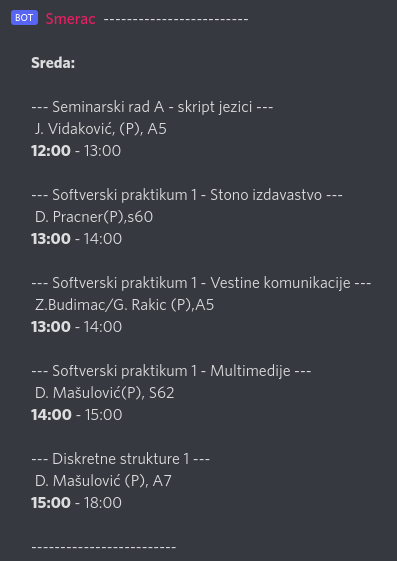
\includegraphics[width=6cm]{sreda}
     \caption{Generisan raspored časova za sredu}
     \label{fig:raspored}
   \end{minipage}\hfill
   \begin{minipage}{0.48\textwidth}
     \centering
     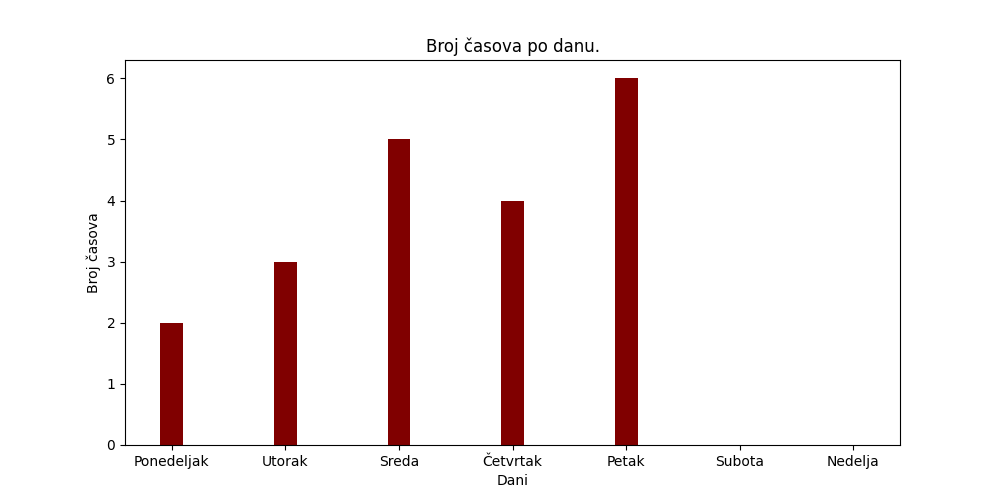
\includegraphics[width=8cm]{it}
     \caption{Grafik sa dnevnim prikazom časova}
     \label{fig:grafik}
   \end{minipage}
\end{figure}
\vfill
\newpage

\section{Opis programa}
\subsection{Nagli prekid usled greške}
Deo koda prikazan na Listingu \ref{lst:fail} služi da prekine tok programa u potpunosti, najčešće se koristi prilikom učitavanja promenjlivih okruženja tj. u slučaju da nisu postavljene.
\begin{lstlisting}[language=Python, caption=Nagli prekid usled greške, label=lst:fail]
    def fail(msg):
        print(msg)
        exit(1)
\end{lstlisting}
\subsection{Promenljive okruženja}
Da bi Smerač mogao učitati potrebne postavke, koristi se biblioteka \textit{OS}. U kodu prikazanom na Listingu \ref{lst:env} se takođe može videti upotreba naglog prekida kao i korišćenje nekih podrazumevanih vrednosti.
\begin{lstlisting}[language=Python, caption=Učitavanje promenljivih okruženja, label=lst:env]
    def setup_config():
        config = dict()

        ...

        COMMAND = os.getenv("COMMAND")
        if COMMAND == None:
            COMMAND = "smer"
        config["command"] = COMMAND

        ...

        DISCORD_TOKEN = os.getenv("DISCORD_TOKEN")
        if DISCORD_TOKEN == None:
            fail("DISCORD_TOKEN env isn't set")
        config["discord_token"] = DISCORD_TOKEN

        NUMBER_OF_ROLES = int(os.getenv("NUMBER_OF_ROLES"))
        if NUMBER_OF_ROLES == None:
            fail("NUMBER_OF_ROLES env isn't set")

        ...

        return config
\end{lstlisting}
\newpage
\subsection{Logging}
Jedna od krucijalnih funkcionalnosti svakog programa je mogućnost zapisivanja šta se dešava prilikom izvršavanja. To je najpotrebnija alatka tokom debagovanja starog ili novog koda neke naknadno dodate funkcionalnosti. Podešavanje fajla za logovanje je prikazano na Listingu \ref{lst:logconf} a opcije logovanja na Listingu \ref{lst:log}.
\begin{lstlisting}[language=Python, caption=Podešavanje fajla za logovanje, label=lst:logconf]
def setup_config():
    
    ...

    LOG_FILE = os.getenv("LOG_FILE")
    if LOG_FILE == None:
        LOG_FILE = "/config/logs/%s.log"%(datetime.today().strftime("%Y-%m-%d-%H-%M-%S"))
    config["log_file"] = LOG_FILE
    
    ...
\end{lstlisting}
\begin{lstlisting}[language=Python, caption=Opcije loga, label=lst:log]
def setup_logger(config):
    if os.getenv("DEBUG") == None:
        logging_level = logging.INFO
    else:
        logging_level = logging.DEBUG

    logging.basicConfig(
        filename=config["log_file"],
        level=logging_level,
        format=
        "%(asctime)s - %(name)s[%(process)s] - %(levelname)s - %(message)s",
    )
\end{lstlisting}
\subsection{Globalne promenljive}
Globalne promenljive su potrebne isključivo kada više različitih funkcija zahtevaju čitanje i pisanje zajedničkih podataka. Odličan primer ovoga bi bila konfiguracija sa svim postavkama potrebnim za rad programa prikazana na Listingu \ref{lst:global}. Pored toga, koristi se i promenljiva \texttt{log} i \texttt{bot} koja služi da interaguje sa interactions-py API.
\begin{lstlisting}[language=Python, caption=Globalne promenljive, label=lst:global]
log = logging.getLogger("smerac")
config = setup_config()
bot = interactions.Client(token=config["discord_token"])
\end{lstlisting}
\newpage
\subsection{Slash komande}
\textit{Slash komande} se zapisuju u obliku:
\begin{verbatim}
    /<naziv_komande> [opcija_1] [opcija_2] ...
\end{verbatim}
Takve komande su standardizovan način pozivanja funkcija proizvoljnog Discord bota.
\subsubsection{Kreiranje slash komande}
Pomoću biblioteke interactions-py moguće je kreirati slash komandu sa nazivom \texttt{smer} i obaveznom opcijom \texttt{wanted\_role} što je prikazano na Listingu \ref{lst:botcommand}. Na Slici \ref{fig:slashcommand} vidljiv je izgled komande korisnicima na Discordu.
\vfill
\begin{lstlisting}[language=Python, caption=Kreiranje slash komande, label=lst:botcommand]
@bot.command(
    name="smer",
    description="Choose your role!",
    options = [
        interactions.Option(
            name="wanted_role",
            description="The role you want.",
            type=interactions.OptionType.STRING,
            required=True,
        ),
    ],
)
\end{lstlisting}
\vfill
\begin{figure}[!htb]
    \centering
    
\includegraphics[width=6cm]{slashcommand}
    \caption{Slash komanda na Discordu}
    \label{fig:slashcommand}
\end{figure}
\vfill
\newpage
\subsubsection{Dodeljivanje funkcionalnosti slash komandi}
Da bi kreirana slash komanda izvršavala neki kod potrebno je odmah ispod njene kreacije deklarisati asinhrohu funkciju, prikazanu na Listingu \ref{lst:chooserole}, koja će izvršavati željeni kod. Ova funkcija prolazi kroz sve smerove autora komande i briše ih a potom dodaje samo željenu.
\begin{lstlisting}[language=Python, caption=Dodeljivanje funkcionalnosti slash komandi, label=lst:chooserole]
async def choose_role(ctx: interactions.CommandContext, wanted_role: str):
    author = ctx.author

    log.debug(f"Started choosing role for {author.nick}")

    guild = await ctx.get_guild()
    discord_roles = await guild.get_all_roles()

    for author_role_id in author.roles:
        author_role = await guild.get_role(author_role_id)
        for role in config["roles"]:
            if role.upper() == author_role.name.upper():
                await author.remove_role(author_role_id)
                log.debug(f"Removed {author.nick} from {role}")
            else:
                log.debug(f"Role {role} isn't {author_role.name}")
    
    if wanted_role != "none":
        for role in config["roles"]:
            if wanted_role.upper() == role.upper():
                for discord_role in discord_roles:
                    if wanted_role.upper() == discord_role.name.upper():
                        await author.add_role(discord_role.id)
                        break
                break
        log.info(f"Added {author.nick} to {wanted_role}.")
        await ctx.send(f"Succesfully added {author.nick} to {wanted_role.upper()}!", ephemeral=True)
    else:
        log.info(f"Removed {author.nick} from all roles.")
        await ctx.send(f"Succesfully removed {author.nick} from all roles!", ephemeral=True)
\end{lstlisting}
Opcija \textit{ephemeral} znači da se poruka šalje samo autoru komande, tj. korisniku koji je pozvao komandu za izmenu smera.
\newpage
\subsection{Kalendar}
\subsubsection{Instanciranje niti}
Kako bi se kalendar asinhrono učitavao za svaki od smerova odvojena je funkcija koja pronalazi sve kanale sa nazivom smera u kategoriji \texttt{calendar}, prikazana na Listingu \ref{lst:threads}, od funkcije za učitavanje, parsiranje i generisanje kalendara.
\begin{lstlisting}[language=Python, caption=Instanciranje niti, label=lst:threads]
async def calendar(delay):
    log.debug("Calendar")

    for guild in bot.guilds:
        channels = await guild.get_all_channels()
        for category in channels:
            if category.type == interactions.ChannelType.GUILD_CATEGORY and category.name.upper() == "calendar":
                for role in config["roles"]:
                    for channel in channels:
                        if channel.parent_id == category.id and role.upper() == channel.name.upper():
                            CALENDAR_URL = os.getenv("CALENDAR_URL_" + role)
                            if CALENDAR_URL == None:
                                log.info("CALENDAR_URL_%s env isn't set, skipping."%(role))
                            else:
                                asyncio.create_task(updateCalendar(channel, CALENDAR_URL, delay))
                            break
                break
\end{lstlisting}
U slučaju da ne postoji URL za kalendar proizvoljnog smera, program beleži to u log i nastavlja da se izvršava.
\newpage
\subsubsection{Ažuriranje kalendara}
Glavna funkcija, prikazana na Listingu \ref{lst:update}, se bavi pozivom svih pomoćnih za rad sa kalendarom. Učitava JSON objekat sa URL-a u \texttt{calendar} rečnik, generiše narednu sedmicu u \texttt{week\_data} i parsira je za podatke u \texttt{week}. \texttt{week\_data} i \texttt{week} su rečnici sačinjeni iz polja sa imenima svih dana u sedmici gde je svaki od njih lista događaja tj. predavanja. Na kraju vrši ispis parsirane sedmice, ako se razlikuje od prošle sedmice tj. \texttt{week\_old}, i takođe šalje sliku grafa sa brojem časova po danu.
\begin{lstlisting}[language=Python, caption=Ažuriranje kalendara, label=lst:update]
async def updateCalendar(channel, calendar_url, delay):
    log.debug("Updating calendar for " + channel.name)
    spacer = "-------------------------"
    week_old = dict()
    while True:
        calendar = json.loads(requests.get(calendar_url).text)
        week_data = await generateWeek(calendar["items"])
        week = await parseWeek(week_data)
        if week_old != week:
            log.debug(str(week_old))
            log.debug("----- week_old != week -----")
            log.debug(str(week))
            week_old = week
            await channel.purge(8, check=check_pinned)
            for weekday in week:
                if week[weekday] != []:
                    day_output = spacer
                    day_output += "\n\n**" + dayInWeekSrpski(weekday) + ":**\n\n"
                    for event in week[weekday]:
                        day_output += "--- " + event["name"] + " ---\n"
                        for info in event["info"]:
                            day_output += info["name"] + "\n"
                            for i in range(len(info["start_times"])):
                                day_output += "**" + info["start_times"][i] + "** - " + info["end_times"][i] + "\n"
                        day_output += "\n"
                    day_output += spacer
                    await channel.send(content=day_output)
            await channel.send(files = await classesPerDayGraph(channel.name, week))
        await asyncio.sleep(delay)
\end{lstlisting}
\newpage
\subsubsection{Generisanje sedmice}
Funkcija, prikazana na Listingu \ref{lst:generate}, prolazi kroz raspored za celu godinu (JSON objekat) i uzima sve događaje koji se odvijaju u narednih 7 dana. Zatim ih svrstava po danima u rečnik \texttt{week} sačinjenen iz polja sa imenima svih dana u sedmici gde je svaki od njih lista događaja tj. predavanja i sortira događaje po početnom vremenu odvijanja. Na kraju vraća rečnik \texttt{week}.
\begin{lstlisting}[language=Python, caption=Generisanje sedmice, label=lst:generate]
async def generateWeek(events):
    log.debug("Generating week")

    current_date = date.today()
    week = {"mon": [], "tue": [], "wed": [], "thu": [], "fri": [], "sat": [], "sun": []}

    for event in events:
        start_date = datetime.fromisoformat(event["start"]["dateTime"]).date()
        if (start_date >= current_date) and (start_date < current_date + timedelta(days=7)):
            week[dayInWeek(start_date.weekday())].append(event)

    for weekday in week:
        week[weekday].sort(key = lambda event : datetime.fromisoformat(event["start"]["dateTime"]))

    return week
\end{lstlisting}
\newpage
\subsubsection{Parsiranje sedmice}
Funkcija, prikazana na Listingu \ref{lst:parse}, prolazi kroz sedmicu i spaja duplikate časova u rečnik \texttt{week} koji je sačinjenen iz polja sa imenima svih dana u sedmici gde je svaki od njih lista događaja tj. predavanja, ali razlikuje ako isti čas drže različiti profesori ili se odvija na drugom mestu.
\\\\
Smerač postiže to razlikovanje deljenjem polja \texttt{summary} na \texttt{name} (sve pre prve zapete) tj. naziv događaja i ostatak \texttt{info} koji predstavlja sve informacije o događaju kao što su mesto odvijanja i ime profesora ili asistenta. Nakon te podele briše sve bele praznine (eng. \textit{white spaces}) i proverava da li u parsiranoj sedmici (rečnik \texttt{week}) već postoji događaj sa tim nazivom, ako postoji proverava se da li postoji isti \texttt{info} unutar tog događaja. Ako se naiđe na iste informacije samo se dodaju nova vremena odvijanja (početak i kraj). U slučaju da se ne pronađe već postojeći događaj ili unutar događaja informacije onda se one kreiraju.
\\\\
Ovakvim parsiranjem rečnik \texttt{week} ima sledeću strukturu:
\begin{center}
\begin{tabular}{|p{1.3cm}|p{1.4cm}|p{1.55cm}|p{2cm}|p{1.9cm}|p{2cm}|p{1.8cm}|}
    \hline
    weekday & event & name & info & info name & start\_times & end\_times \\
    \hline
    [event] & \{name, info\} & 'string' & \{name, start\_times, end\_times\} & 'string' & ['\%H:\%M'] & ['\%H:\%M'] \\
    \hline
\end{tabular}
\end{center}
'\%H:\%M' predstavlja string koji je konvertovan iz \texttt{datetime} ISO formata u obliku SAT : MINUT.
\newpage
\begin{lstlisting}[language=Python, caption=Parsiranje sedmice, label=lst:parse]
async def parseWeek(week_data):
    log.debug("Parsing week")
    week = {"mon": [], "tue": [], "wed": [], "thu": [], "fri": [], "sat": [], "sun": []}
    for weekday in week_data:
        if week_data[weekday] != []:
            for event in week_data[weekday]:
                name, info = event["summary"].split(",", 1)
                start_time = datetime.fromisoformat(event["start"]["dateTime"]).strftime("%H:%M")
                end_time = datetime.fromisoformat(event["end"]["dateTime"]).strftime("%H:%M")
                foundEvent = False
                if week[weekday] != []:
                    for event_old in week[weekday]:
                        if name.upper().replace(" ", "") == event_old["name"].upper().replace(" ", ""):
                            foundInfo = False
                            for info_old in event_old["info"]:
                                if info.upper().replace(" ", "") == info_old["name"].upper().replace(" ", ""):
                                    info_old["start_times"].append(start_time)
                                    info_old["end_times"].append(end_time)
                                    foundInfo = True
                                    break
                            if not foundInfo:
                                new_info = {"name": info, "start_times": [], "end_times": []}
                                new_info["start_times"].append(start_time)
                                new_info["end_times"].append(end_time)
                                event_old["info"].append(new_info)
                            foundEvent = True
                            break
                if not foundEvent:
                    new_event = {"name": name, "info": []}
                    new_info = {"name": info, "start_times": [], "end_times": []}
                    new_info["start_times"].append(start_time)
                    new_info["end_times"].append(end_time)
                    new_event["info"].append(new_info)
                    week[weekday].append(new_event)
    return week
\end{lstlisting}
\newpage
\subsection{Kreiranje grafa}
Funkcija, prikazana na Listingu \ref{lst:graph}, prolazi kroz parsiranu sedmicu i broji koliko ima časova po danu, nakon toga generiše graf uz pomoć matplot\cite{matplotlib} biblioteke. Povratna vrednost je lokacija sačuvane slike grafa.
\begin{lstlisting}[language=Python, caption=Kreiranje grafa, label=lst:graph]
async def classesPerDayGraph(channel_name, week):
    log.debug("Plotting graph for " + channel_name)

    filename = config["saved_plots"] + "/" + channel_name + ".png"
    data = dict()

    for weekday in week:
        data[dayInWeekSrpski(weekday)] = len(week[weekday])

    keys = list(data.keys())
    values = list(data.values())

    fig = plt.figure(figsize = (10, 5))

    plt.bar(keys, values, color ='maroon', width = 0.2)

    plt.xlabel("Dani")
    plt.ylabel("Broj casova")
    plt.title("Broj casova po danu.")

    plt.savefig(filename)
    plt.close()

    return interactions.File(filename=filename)
\end{lstlisting}
\newpage
\section{Zaključak}
Pored toga što je Smerač projekat za uspešno polaganje predmeta Skript jezici, to je i društveno korisna aplikacija koja se koristi na Discord serveru studenata Departmana za matematiku i informatiku. Najpre nudi jednostavan i bezbedan način odabira smera što smanjuje potrebu za ručnim radom neke privilegovane osobe ali i ubrzava čitav proces. Prilikom odabira smera studenti dobijaju pristup isključivo onim kanalima koji su potrebni za taj smer i time se olakšava pregled i upotreba Discord servera. Naravno, najkompleksnija funkcionalnost ovog programa jeste parsiranje kalendara, ali nakon što je ta prepreka pređena studentima je dostupan drastično brži i lakši pristup rasporedu predavanja i vežbi.
\\\\
Smerač je takođe slobodnog i otvorenog koda i kao takav može biti uzor drugim aplikacija sličnog tipa, što i jeste slučaj za budući projekat jednog studenta koji planira da integriše Moodle notifikacije vezane za smer i prosledi ih na isti Discord server.
\newpage

\pagestyle{plain}
\renewcommand\refname{Literatura}
\addcontentsline{toc}{section}{Literatura}
\bibliography{references}
\bibliographystyle{ieeetr}

\end{document}